%%%%%%%%%%%%%%%%%%%%%%%%%%%%%%%%%%%%%%%%%
% 
% LaTeX Template
% Version 3.1 (25/3/14)
%
%%%%%%%%%%%%%%%%%%%%%%%%%%%%%%%%%%%%%%%%%

%----------------------------------------------------------------------------------------
%	PACKAGES AND DOCUMENT CONFIGURATIONS
%----------------------------------------------------------------------------------------

\documentclass[12pt, a4 paper]{article}

\usepackage{tikz}
%\usepackage[top=2cm, bottom=2cm, outer=0cm, inner=0cm]{geometry}
\usepackage{graphicx} % Required for the inclusion of images
\usepackage{multicol} % Required for multicolumns
\usepackage{setspace} % Required for line spacing
\setlength\parindent{0pt} % Removes all indentation from paragraphs
\setlength{\columnseprule}{0.4pt} % Adds vertical line between multicolumns
\usepackage{multirow} % Required for multirows
\usepackage{booktabs} % For prettier tables
\usepackage{xcolor}
%\usepackage{tabularx}
%\renewcommand{\rmdefault}{ptm}

%\usepackage{helvet}

\usepackage{times} % Uncomment to use the Times New Roman font

%----------------------------------------------------------------------------------------
%	DOCUMENT INFORMATION
%----------------------------------------------------------------------------------------

\begin{document}

\tikz[remember picture,overlay] \node[inner sep=0pt] at (current page.center){
\includegraphics[width=\paperwidth,height=\paperheight]{image.jpeg}};

\clearpage

%\font\myfont=cmr12 at 35pt
%\title{\myfont  Event Name} % Write Event name here
%\author{}
%\date{\vspace{-10ex}}

%\maketitle % Insert the title, author and date
\setstretch{1.5}

\tikz[remember picture,overlay] \node[opacity=0.8,inner sep=0pt] at (current page.center){
\includegraphics[width=\paperwidth,height=\paperheight]{Border48-A4--Arvin61r58.png}};
%\tikz[remember picture,overlay] \node[opacity=0.5,inner sep=0pt] at (current page.center){\includegraphics[width=\paperwidth,height=\paperheight]{color-2174049__340.png}};

\begin{center}
\Huge \bfseries \ttfamily SEMINAR ON RESEARCH PAPER WRITING AND PUBLISHING
\end{center}

\begin{center}
\large A Seminar on how to write a research paper 
\end{center}

\begin{center}
\begin{multicols}{2}
\begin{tabular}{l r}
Date: & 04/04/2019\\ % Date the event was held
Time: & 4:00 P.M to 5:30 P.M \\ % Time of event 
\end{tabular}
\columnbreak
\begin{tabular}{l r}
Venue: & Workshop Seminar Hall \\ % Venue of event
%Total Attendance: & Number \\ % Number of participants
\end{tabular}
\end{multicols}

\begin{Large}
%\begin{multicols}{2}
A seminar on Research paper writing and publishing was organized on April 04,2019 from 4:00 pm to 5:30 p.m. in workshop seminar hall of the college. This session was organised to guide students about research paper and publishing related doubts .
%\columnbreak
%\includegraphics[width=\linewidth]{placeholder.jpg}
  %\caption{A boat.}
  %\label{fig:boat1}
%\end{multicols}

%\begin{multicols}{2}

%\includegraphics[width=\linewidth]{placeholder.jpg}

%\columnbreak
 The session was delivered by DR.ARVIND DHINGRA.Sir cleared the doubts of students regarding the publishing and  research paper writing. 
%\end{multicols}

\newpage 

\tikz[remember picture,overlay] \node[opacity=0.8,inner sep=0pt] at (current page.center){
\includegraphics[width=\paperwidth,height=\paperheight]{5TRrp44jc.png}};
%\tikz[remember picture,overlay] \node[opacity=0.8,inner sep=0pt] at (current page.center){\includegraphics[width=\paperwidth,height=\paperheight]{md_5b0912b7c0870.png}};

%\begin{multicols}{2}
Sir told the students that while writing a Research Paper one should keep in mind about 'Plagiarism' i.e. Sometimes we copy the thoughts of others unknowingly and thus this is a great loss.Also while writing the research paper one can refer to various journals and also refer to internet.
%\columnbreak
%\includegraphics[width=\linewidth]{placeholder.jpg}
  
%\end{multicols}

%\begin{multicols}{2}
%\includegraphics[width=\linewidth]{placeholder.jpg}

%\columnbreak
Sir also shared his own experience of writing the research paper. He then wrapped the session by encouraging students to write either their own research paper  or in a group whatever way is suitable to them.
  
%\end{multicols} 

%\begin{multicols}{2}
%Some paragraph

%\columnbreak
%\includegraphics[width=\linewidth]{placeholder.jpg}
  
%\end{multicols} 

%\begin{multicols}{2}
%\includegraphics[width=\linewidth]{placeholder.jpg}

%\columnbreak
%Some paragraph
  
%\end{multicols} 

\end{Large} 
\end{center}

\newpage 

\tikz[remember picture,overlay] \node[opacity=0.8, inner sep=0pt] at (current page.center){
\includegraphics[width=\paperwidth,height=\paperheight]{5TRrp44jc.png}};
%\tikz[remember picture,overlay] \node[opacity=0.8,inner sep=0pt] at (current page.center){\includegraphics[width=\paperwidth,height=\paperheight]{md_5b0912b7c0870.png}};

\begin{center}
\Huge Pictures Section
 
\tikz[remember picture,overlay] \node[opacity=0.8,inner sep=0pt] at (current page.center){
\includegraphics[width=\paperwidth,height=\paperheight]{5TRrp44jc.png}};
%\tikz[remember picture,overlay] \node[opacity=0.8,inner sep=0pt] at (current page.center){\includegraphics[width=\paperwidth,height=\paperheight]{md_5b0912b7c0870.png}};

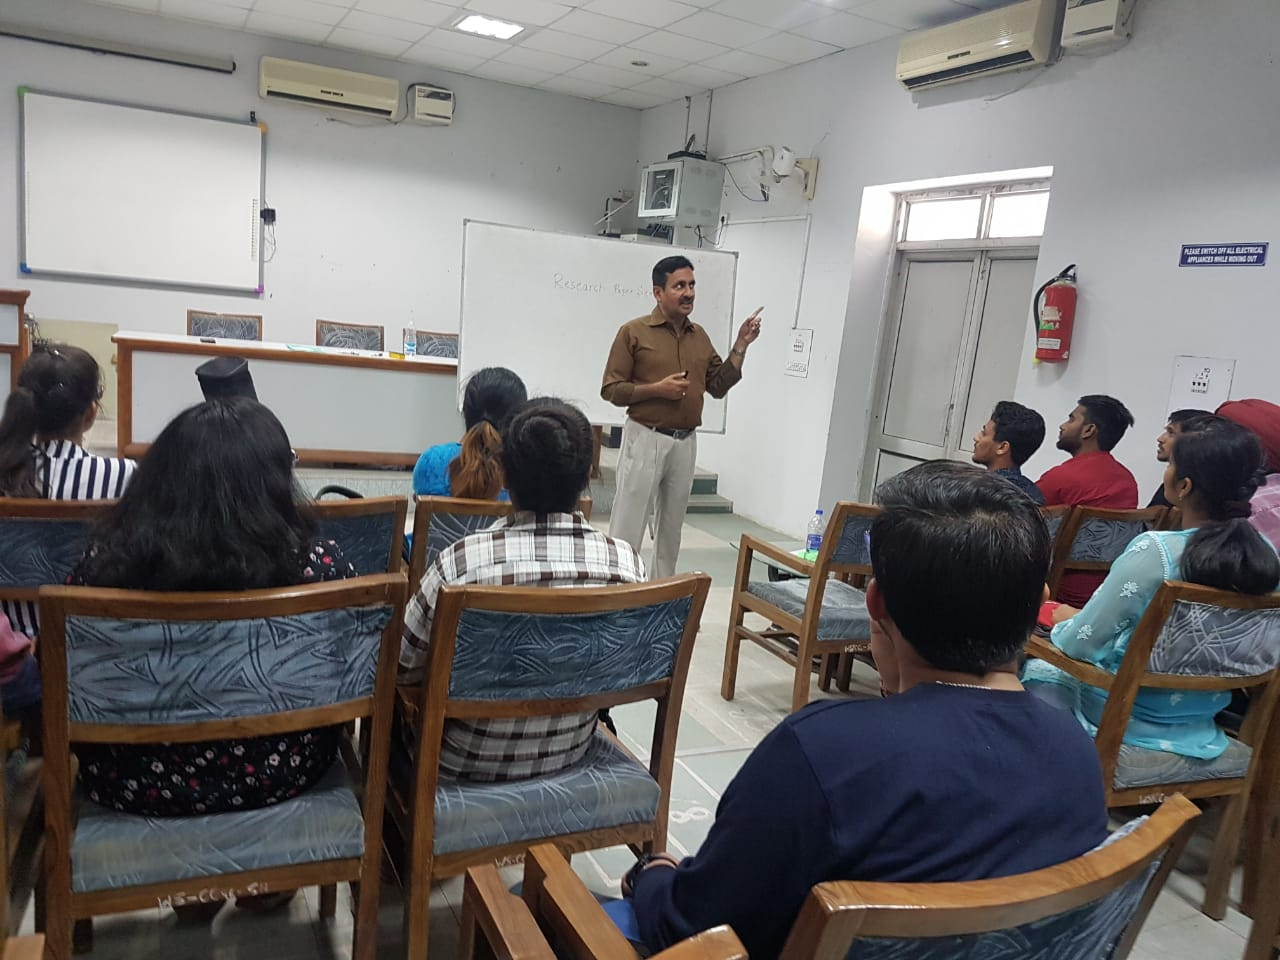
\includegraphics[height=5cm]{image1.jpg}

\medskip\medskip

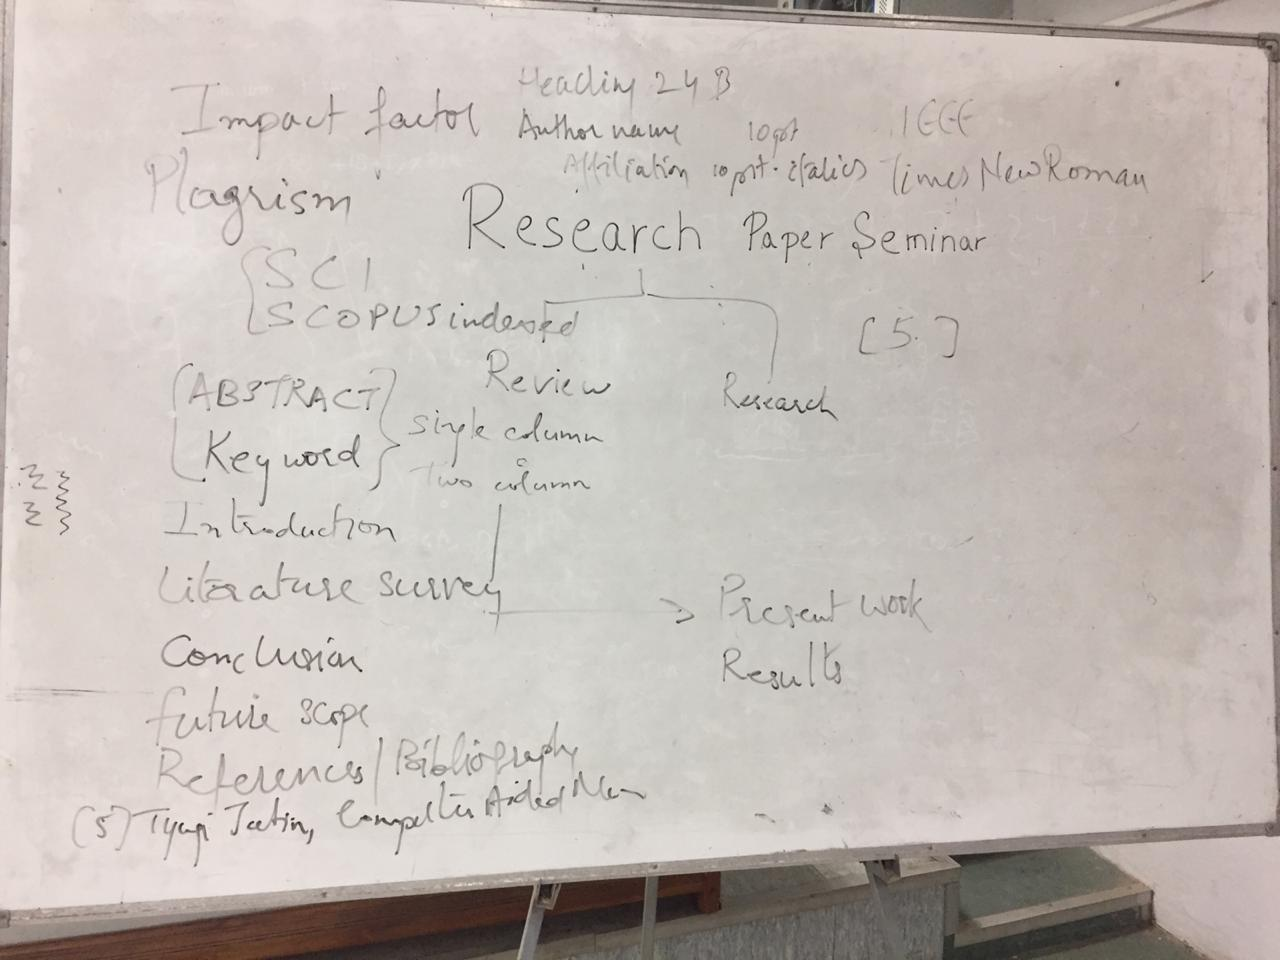
\includegraphics[height=5cm]{image2.jpeg}

\medskip\medskip

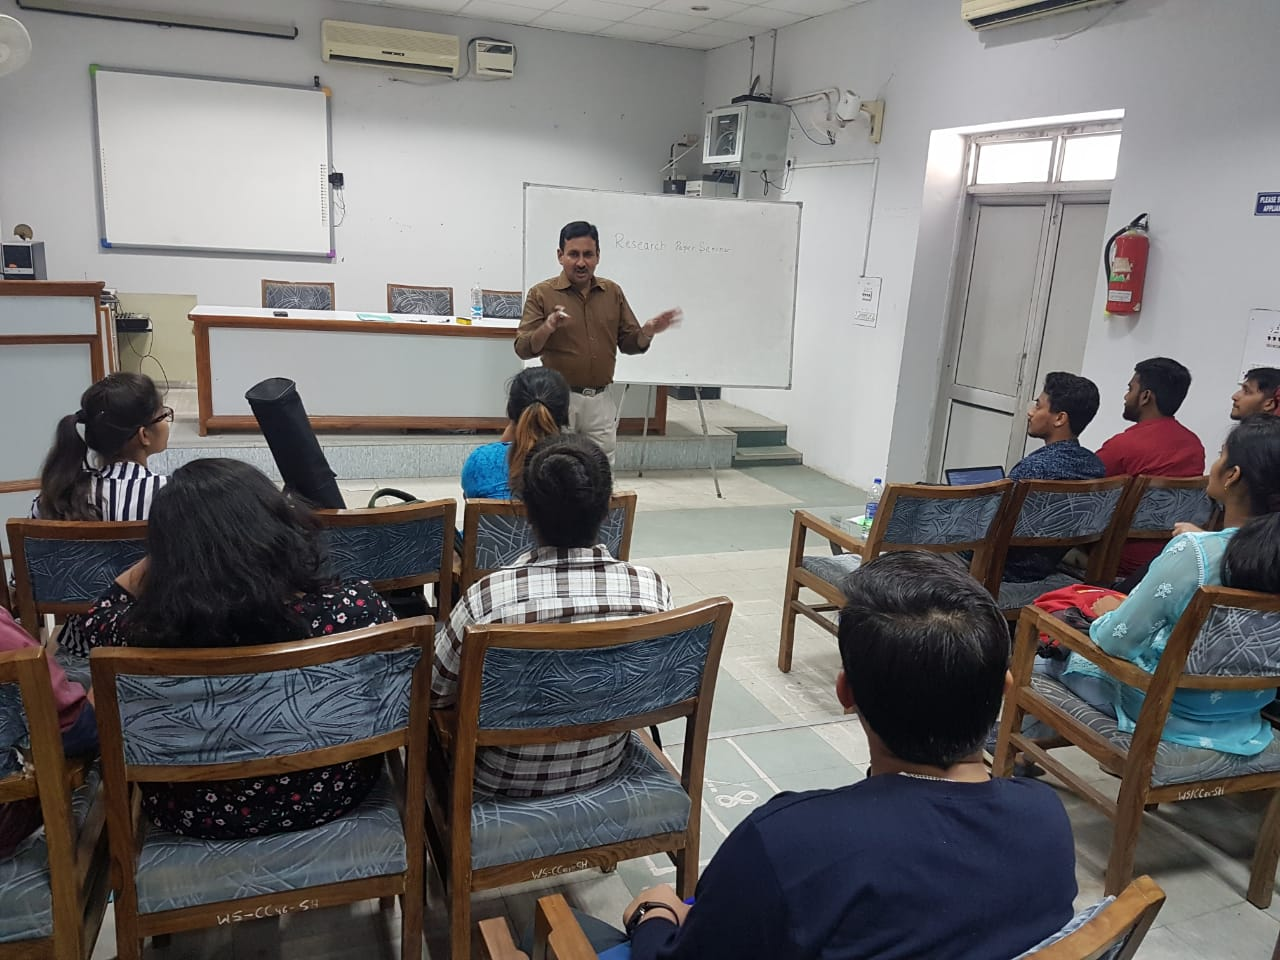
\includegraphics[height=5cm]{image3.jpg}

\end{center}

\begin{center}
\huge Organisers list
\end{center}

\begin{table}[h!]
  \begin{center}
    \begin{tabular}{|c|c|c|c|c|c|} 
    \toprule % <-- Toprule here
      \textbf{S.No.} & \textbf{Name} & \textbf{Branch/Year} & \textbf{U.R.N} \\
      \midrule % <-- Midrule here
      1 & MANOOR KAUR	   & D4 IT	& 1507942 \\
      2	& MANVEER KAUR	   & D4 CSE	& 1507620 \\
      3	& KANWARDEEP SINGH & D4 IT	& 1507934 \\
      4	& PARIDHI	       & D2 CSE	& 1706485 \\
      5	& KAVISH	       & D1 IT	& 1805520 \\
      6	& PAWAN	           & D1 ECE	& 1805429 \\
      7	& RAHUL	           & D1 IT	& 1805543 \\
      8	& DOLLY KUMARI	   & D1 IT  & 1805504 \\

      \bottomrule % <-- Bottomrule here
    \end{tabular}
  \end{center}
\end{table}

\tikz[remember picture,overlay] \node[opacity=0.8,inner sep=0pt] at (current page.center){
\includegraphics[width=\paperwidth,height=\paperheight]{5TRrp44jc.png}};
%\tikz[remember picture,overlay] \node[opacity=0.8,inner sep=0pt] at (current page.center){\includegraphics[width=\paperwidth,height=\paperheight]{md_5b0912b7c0870.png}};



\end{document}